\ifdefined\maindoc
% Under the thesis build, main.tex owns the full \graphicspath list. \graphicspath REPLACES
% rather than appends, so this branch deliberately does nothing.
\else
\documentclass[12pt]{report}
\usepackage[a4paper,margin=1in]{geometry}
\usepackage[utf8]{inputenc}
\usepackage[T1]{fontenc}
\usepackage[british]{babel}
\usepackage{amsmath,amssymb,amsthm}
\usepackage{booktabs}
\usepackage{setspace}
\usepackage{graphicx}
\usepackage{subcaption}
\usepackage{enumitem}
\usepackage{placeins}
\usepackage{hyperref}
\usepackage{array}
\usepackage{algorithm}
\usepackage{algpseudocode}
\usepackage[backend=biber,style=ieee,citestyle=numeric-comp,sorting=none]{biblatex}
\addbibresource{../../references.bib}
\newtheorem{theorem}{Theorem}
\newtheorem{lemma}[theorem]{Lemma}
\newtheorem{definition}[theorem]{Definition}
\newtheorem{proposition}[theorem]{Proposition}
\onehalfspacing
\graphicspath{{figures/}}
% Standalone-only fallbacks. Numbering: 1 Introduction, 2 Background, 3 Network Model,
% 4 Network Decomposition, 5 Probability, 6 Capacity Flow, 7 this chapter, 8 Julia package,
% 9 Interface, 10 Integrated Case Study, 11 Conclusions.
\makeatletter
\newlabel{ch:lit-review}{{2}{1}{}{Doc-Start}{}}
\newlabel{ch:system-model}{{3}{1}{}{Doc-Start}{}}
\newlabel{ch:diamond-module}{{4}{1}{}{Doc-Start}{}}
\newlabel{ch:probability-toolkit}{{5}{1}{}{Doc-Start}{}}
\newlabel{ch:julia-package}{{8}{1}{}{Doc-Start}{}}
\newlabel{ch:conclusions}{{11}{1}{}{Doc-Start}{}}
\newlabel{app:network-specs}{{A}{1}{}{Doc-Start}{}}
\newlabel{app:full-results}{{B}{1}{}{Doc-Start}{}}
\makeatother
\begin{document}
\title{Information as Schedule and Cost: Critical Path Toolkit}
\fi

\newcommand{\comb}{\oplus}
\newcommand{\prop}{\otimes}
% Placeholder for numbers awaiting the PSPLIB and drone-design runs. Renders in bold
% brackets so nothing can be mistaken for a result.
\providecommand{\PH}[1]{\textbf{[#1]}}

\section{Introduction}
\label{sec:cpm-intro}

This chapter presents the Critical Path Toolkit, which implements the schedule and cost
reading of the network model. In this reading the value attached to a node is a quantity
that accumulates along dependency paths, such as a duration or a cost, and the value attached to an edge is the amount added or applied in the transfer
between two components. The toolkit reads the graph object of
Chapter~\ref{ch:system-model} directly. Every analysis in it is a linear-time pass over the
layered iteration sets, and the Network Decomposition Module of
Chapter~\ref{ch:diamond-module} is not used.

For a network carrying such a quantity, a forward pass gives the best or worst value that a
complete chain of dependencies can produce. The margin of a component is how far it can
move before that value changes. The margin identifies the critical components, and it can be computed only when the arithmetic of
the quantity can be run backwards.

The contributions of this chapter are the following. The classical critical path method is
generalised to a family of analysis modes, each defined by a pair of operators, and the
condition under which a mode has a backward pass is stated and used to select the modes
provided. Two propagation kernels are given that serve every mode. For interval durations,
the forward quantities are computed exactly from two corner runs, and the floats are
computed exactly by a domination split that reduces the enumeration from every uncertain
duration to those that can bypass the node in question. Every result is checked against an
independent oracle.

The rest of the chapter is structured as follows. Section~\ref{sec:cpm-grounding} recalls
the results from Chapter~\ref{ch:lit-review} on which the toolkit builds.
Section~\ref{sec:cpm-modes} defines the analysis modes and Section~\ref{sec:cpm-kernels}
the two kernels. Section~\ref{sec:cpm-interval} describes the treatment of interval
durations, and Section~\ref{sec:cpm-split} presents the domination split and proves its
exactness. Section~\ref{sec:cpm-validation} describes the validation of the toolkit.
Section~\ref{sec:cpm-cases} applies it to a benchmark project network and locates the
boundary of the split on a dense mesh.
Section~\ref{sec:cpm-discussion} discusses limitations and extensions, and
Section~\ref{sec:cpm-summary} concludes the chapter.

\section{Background}
\label{sec:cpm-grounding}

Chapter~\ref{ch:lit-review} reviewed the critical path method \cite{kelley1959critical},
its float calculus, and the treatment of duration uncertainty from PERT
\cite{malcolm1959pert} to the interval results of Chanas, Zieli\'{n}ski and their
co-authors. When each duration is an interval, the forward quantities are monotone in the durations,
and their exact bounds are found at the two corners of the input box. The backward
quantities are not monotone. Deciding whether an activity is possibly critical is
NP-complete and computing float bounds is NP-hard
\cite{chanas2002complexity,chanas2003planar,dubois2005floats,fortin2010criticality}. The
interval treatment of Sections~\ref{sec:cpm-interval} and~\ref{sec:cpm-split} rests on
these two facts.

The forward and backward passes of the classical method are linear algebra over an
idempotent semiring, and the backward pass is a residuation \cite{baccelli1992sync}.
Hence a forward recursion exists for any pair of combination and compounding operations,
but a backward pass exists only when the algebra of the pair supports one. A slack
reported for a pair without such a backward pass is a number with no meaning. The modes of
Section~\ref{sec:cpm-modes} rest on this fact.

\section{Analysis Modes}
\label{sec:cpm-modes}

The forward recursion of the critical path method combines the values arriving at a node
from its parents and compounds the result with the node's own value. Writing $\comb$ for
the combination and $\prop$ for the compounding, the classical method has $\comb = \max$
and $\prop = +$. Other pairs give other analyses: $\min$ and $+$ give the fastest chain,
$\max$ and $\times$ give the best multiplicative chain, and $+$ and $+$ give a roll-up in
which every route contributes. Whether a margin is defined is a property of the pair.

When $\comb$ is an order ($\max$ or $\min$) and $\prop$ is monotone with a residual, it
is. A bound on the combined value then binds every argument, and the bound inverts
across each edge, so a constraint of the form ``finish by $K$'' travels backwards through
the network in the same way that values travel forwards. This is residuation in an
idempotent semiring \cite{baccelli1992sync}, and it is what the classical backward pass
is. The backward object is a margin: the distance between the best complete path and the
best complete path forced through the node in question, expressed as a difference for the
additive pairs and as a ratio for the multiplicative one. The zero set of the margin is
the critical structure of the analysis.

When $\comb$ is a sum, a total is not a deadline and no residuation exists. However, a
summed system is linear, and a linear map has an adjoint. The backward object
is therefore a sensitivity, and the margin it defines is an allowance against a stated
budget. It is not a slack against a deadline. A pair with neither structure supports a forward
recursion and nothing else, and no margin is defined for it.

A configuration of the toolkit is called a mode. A mode is an operator pair together with
the backward semantics its algebra supports. Table~\ref{tab:cpm-modes} lists the four
modes provided. The MaxScaling mode is applied in Chapter~\ref{ch:integrated-case-study}. The three order-based modes share one kernel and one backward mechanism,
described in Section~\ref{sec:cpm-kernel-order}. The accumulation mode has its own kernel,
described in Section~\ref{sec:cpm-kernel-linear}.

\begin{table}[htbp]
\centering
\caption{The modes provided by the toolkit. In the three order-based modes the backward
quantities are computed by the same fold on the reversed graph and the margin is the gap
between the project value and the value through the node. In the accumulation mode the
backward quantity is the adjoint, a path count.}
\label{tab:cpm-modes}
\small
\renewcommand{\arraystretch}{1.2}
\begin{tabular}{lllll}
\toprule
Mode & $\comb$ & $\prop$ & Backward object & Margin \\
\midrule
LongestPath & $\max$ & $+$ & reverse fold, margin $P - t_v$ & slack \\
ShortestPath & $\min$ & $+$ & reverse fold, margin $t_v - P$ & margin over optimum \\
MaxScaling & $\max$ & $\times$ & reverse fold, margin $P/t_v - 1$ & ratio slack \\
Accumulation & $+$ & $+$ & adjoint (path multiplicity) & allowance under a budget \\
\bottomrule
\end{tabular}
\end{table}

\section{The Propagation Kernels}
\label{sec:cpm-kernels}

\subsection{The order-based kernel}
\label{sec:cpm-kernel-order}

For the order-based modes one fold serves both directions. Let $d_v$ be the value of node
$v$, $w_{uv}$ the value of edge $(u,v)$, $\mathrm{pa}(v)$ the parents of $v$ and
$\mathrm{succ}(v)$ its successors. Read forwards over the layered iteration sets, the fold
computes
\begin{equation}
\label{eq:cpm-forward}
F_v \;=\; \Bigl(\comb_{u \in \mathrm{pa}(v)} \, F_u \prop w_{uv}\Bigr) \prop d_v ,
\end{equation}
the best value that a chain of dependencies can deliver into each node, with each source
seeded from an initial value. Read over the reversed graph, the same fold computes
\begin{equation}
\label{eq:cpm-reverse}
R_v \;=\; \comb_{s \in \mathrm{succ}(v)} \,\bigl(R_s \prop d_s\bigr) \prop w_{vs} ,
\end{equation}
the best completion from each node onwards, with each sink seeded at the neutral element
of $\prop$. The two arrays meet at each node. Their compound
\begin{equation}
\label{eq:cpm-through}
t_v \;=\; F_v \prop R_v
\end{equation}
is the best complete path forced through $v$. The project value $P$ is the combination of
the forward values at the sinks, and the margin of $v$ is the gap between the two,
\begin{equation}
\label{eq:cpm-margin}
m_v = P - t_v \;\;(\text{LongestPath}), \qquad
m_v = t_v - P \;\;(\text{ShortestPath}), \qquad
m_v = P / t_v - 1 \;\;(\text{MaxScaling}).
\end{equation}
A node is critical when its margin is zero. For the additive modes the textbook schedule
quantities are recovered from the same two arrays,
\begin{equation}
\label{eq:cpm-schedule}
\mathrm{ES}_v = F_v - d_v, \qquad \mathrm{LF}_v = P - R_v, \qquad \mathrm{LS}_v = \mathrm{LF}_v - d_v .
\end{equation}
Algorithm~\ref{alg:cpm-order} gives the kernel.

\begin{algorithm}[htbp]
\caption{Order-based kernel (one mode)}
\label{alg:cpm-order}
\begin{algorithmic}[1]
\Require layered iteration sets $L$, incoming and outgoing indices, sources $S$, node
  values $d$, edge values $w$, mode $(\comb, \prop)$ with neutral element $e$
\Ensure $F$, $R$, $P$, $t$, $m$, critical set
\ForAll{layers $L_i$ in order, nodes $v \in L_i$}
  \If{$v \in S$} $F_v \gets e \prop d_v$
  \Else\ $F_v \gets \bigl(\comb_{u \in \mathrm{pa}(v)} F_u \prop w_{uv}\bigr) \prop d_v$
  \EndIf
\EndFor
\ForAll{layers $L_i$ in reverse order, nodes $v \in L_i$}
  \If{$\mathrm{succ}(v) = \varnothing$} $R_v \gets e$
  \Else\ $R_v \gets \comb_{s \in \mathrm{succ}(v)} (R_s \prop d_s) \prop w_{vs}$
  \EndIf
\EndFor
\State $P \gets \comb_{v \in \text{sinks}} F_v$
\ForAll{nodes $v$}
  \State $t_v \gets F_v \prop R_v$; \quad $m_v \gets$ margin$(P, t_v)$ by Eq.~\eqref{eq:cpm-margin}
\EndFor
\State critical $\gets \{\, v : m_v = 0 \,\}$
\end{algorithmic}
\end{algorithm}

On the four-node network of Figure~\ref{fig:cpm-example}, with durations $1, 5, 2, 1$ and
no edge delays, LongestPath completes in $7$ along $1{\to}2{\to}4$ and node $3$ carries
slack $3$. ShortestPath completes in $4$ along $1{\to}3{\to}4$ and node $2$ carries margin
$3$. The two modes select different chains from the same inputs.

\begin{figure}[htbp]
  \centering
  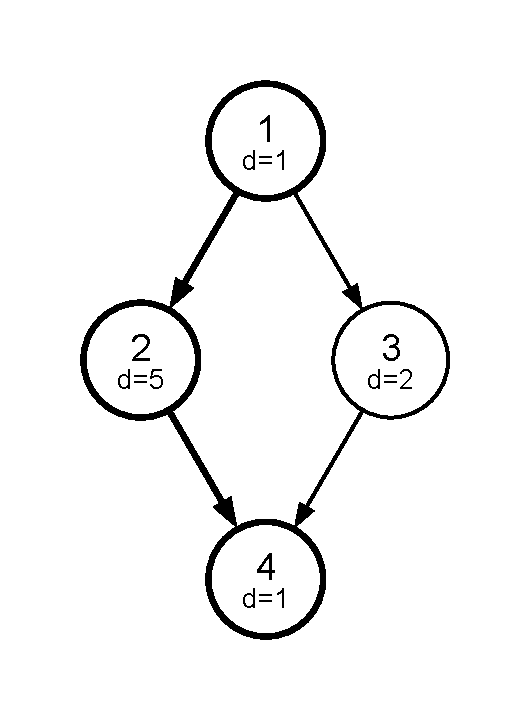
\includegraphics[width=0.3\linewidth]{fig01_example/fig01_example.pdf}
  \caption{The running example. Node durations $1, 5, 2, 1$. LongestPath is critical
  through nodes $1, 2, 4$ and ShortestPath through $1, 3, 4$.}
  \label{fig:cpm-example}
\end{figure}

\subsection{The linear kernel}
\label{sec:cpm-kernel-linear}

In the accumulation mode the combination is a sum, so
\begin{equation}
\label{eq:cpm-acc-forward}
F_v \;=\; \sum_{u \in \mathrm{pa}(v)} \bigl(F_u + w_{uv}\bigr) + d_v .
\end{equation}
A node's value therefore reaches a downstream target once per directed route. The total at
a target $t$ expands to
\begin{equation}
\label{eq:cpm-acc-total}
F_t \;=\; \sum_{v} m_v\, d_v \;+\; \sum_{(u,v) \in E} m_v\, w_{uv} ,
\end{equation}
where $m_v$ is the number of directed routes from $v$ to $t$. The counts are computed by a
reverse traversal seeded with $m_t = 1$,
\begin{equation}
\label{eq:cpm-adjoint}
m_v \;=\; \sum_{s \in \mathrm{succ}(v)} m_s ,
\end{equation}
which is the adjoint of the forward map. The count $m_v$ is the derivative of the total
with respect to the node's value, and the product $m_v d_v$ is the node's contribution to
the total. Under a budget $B$ the allowance of node $v$ is
\begin{equation}
\label{eq:cpm-allowance}
a_v \;=\; \frac{B - F_t}{m_v} ,
\end{equation}
the headroom divided across the node's routes. Algorithm~\ref{alg:cpm-linear} gives the
kernel. On the running example the total at node $4$ is $10$ and node $1$ counts twice,
once through each branch. If no target is given the toolkit takes the sink with the
largest forward value.

\begin{algorithm}[htbp]
\caption{Linear kernel (accumulation mode)}
\label{alg:cpm-linear}
\begin{algorithmic}[1]
\Require layered iteration sets $L$, indices, sources $S$, node values $d$, edge values
  $w$, target $t$ (default: sink with largest $F$), optional budget $B$
\Ensure $F$, total $F_t$, multiplicities $m$, contributions, allowances
\ForAll{layers $L_i$ in order, nodes $v \in L_i$}
  \State $F_v \gets d_v$ if $v \in S$, else $\sum_{u \in \mathrm{pa}(v)} (F_u + w_{uv}) + d_v$
\EndFor
\State $m_t \gets 1$
\ForAll{layers $L_i$ in reverse order, nodes $v \in L_i$, $v \neq t$}
  \State $m_v \gets \sum_{s \in \mathrm{succ}(v)} m_s$
\EndFor
\ForAll{nodes $v$ with $m_v > 0$}
  \State contribution$_v \gets m_v d_v$; \quad if $B$ given, $a_v \gets (B - F_t)/m_v$
\EndFor
\end{algorithmic}
\end{algorithm}

\subsection{Cost}

Both kernels touch each node once and each edge a constant number of times, so every mode
costs $O(|V|+|E|)$ whatever the operators are. The kernels are generic over the value type
they propagate, and the concrete types are described in Chapter~\ref{ch:julia-package}.

\section{Interval Durations}
\label{sec:cpm-interval}

When the durations are intervals, the quantities of the toolkit divide into two classes
according to monotonicity.

Every forward quantity, $F_v$, $R_v$, $t_v$ and $P$, is monotone in every input. Hence its
exact bounds are obtained from two scalar runs of the kernel, one with every input at its
lower endpoint and one with every input at its upper endpoint, and interval arithmetic is
not needed. The toolkit computes the forward quantities in this way for every mode.

A margin is a difference of two monotone quantities that share their inputs, so it is not
monotone in anything, and the hardness results of Section~\ref{sec:cpm-grounding} apply
to it. The toolkit provides three methods for the margins, and each result is tagged with
the method that produced it, so that an exact range and an enclosure cannot be confused.

\begin{enumerate}
\item \emph{Conservative enclosure.} From the exact bounds on $P$ and $t_v$, the LongestPath
  margin lies within
  \begin{equation}
  \label{eq:cpm-enclosure}
  \bigl[\, \max\bigl(0,\; \underline{P} - \overline{t}_v\bigr),\;\; \overline{P} - \underline{t}_v \,\bigr] ,
  \end{equation}
  and correspondingly for the other modes. The enclosure is sound and costs no more than
  the two corner runs. It is not exact, because the lower corner of $P$ and the upper
  corner of $t_v$ are not in general attained by the same configuration of durations.
\item \emph{Exhaustive corner enumeration.} The margin extremes are attained at corner
  configurations (Proposition~\ref{prop:cpm-corner} below), so enumerating every corner of
  the non-degenerate node and edge intervals and running the kernel at each gives the
  exact margin range. The cost is $2^k$ runs for $k$ interval inputs, and the toolkit
  refuses beyond a stated cap unless the cap is raised.
\item \emph{Domination split.} For the LongestPath mode with point-valued edge values, the exact
  margin range is obtained from a much smaller enumeration, described in
  Section~\ref{sec:cpm-split}.
\end{enumerate}

From the margin bounds the toolkit reports the two criticality sets of the interval PERT
literature \cite{chanas2002complexity}. A node is \emph{necessarily critical} when the
upper bound of its margin is zero, that is, it is critical in every configuration of the
box. A node is \emph{possibly critical} when the lower bound of its margin is zero, that
is, it is critical in at least one configuration. Under the conservative enclosure the
necessarily critical set is certain and the possibly critical set is a superset that the
exact methods tighten. Degenerate intervals, whose two endpoints coincide, are held fixed
by every method and do not enter the enumeration.

An earlier implementation of the toolkit ran the scalar kernels on an interval type with
overloaded arithmetic, so that $\max$, $+$ and $-$ were applied to intervals directly. It
was withdrawn because it produced wrong results at the combination and margin steps. In
the combination step,
$\max$ of two overlapping intervals is not defined, since neither contains the other.
Taking the endpoint-wise maximum, which is what the overloaded operator did, returns an
interval such as $[5, 7]$ from $[3, 7]$ and $[5, 6]$, whose lower end comes from one
parent and whose upper end from the other, so the value no longer describes any single
path and the critical chain read from it can be wrong. In the margin step, the float
$P - t_v$ subtracts two quantities that depend on the same durations. Interval
subtraction treats them as independent, which is the dependency problem of
Chapter~\ref{ch:lit-review}. For the dummy start node of a project, for example, $P$ and
$t_v$ are the same interval, say $[30, 46]$, and interval subtraction gives
$[-16, 16]$ when the true float is exactly $0$. The margins were therefore wider than
the true range, and negative floats appeared where none exist. The present toolkit
computes each interval quantity by the scheme its structure permits, and never by
running the kernel on an interval type.

\section{Exact Interval Floats by the Domination Split}
\label{sec:cpm-split}

Throughout this section the mode is LongestPath, the durations $d_u$ lie in intervals,
the edge values are fixed, and $f_v = P - t_v \ge 0$ is the float of node $v$. The
question is the exact range of $f_v$ over the box of duration configurations.

\begin{proposition}[Corner sufficiency]
\label{prop:cpm-corner}
With all other durations fixed, $f_v$ is a monotone function of any single duration
$d_u$. Consequently the extremes of $f_v$ over the box are attained at corner
configurations.
\end{proposition}

\begin{proof}
A path visits a node at most once, so as a function of $x = d_u$ every path length is
either constant or affine with slope one. Hence $P(x) = \max(C_0,\, C_1 + x)$, where $C_1$
is the best path through $u$ and $C_0$ the best avoiding it, and likewise
$t_v(x) = \max(A_0,\, A_1 + x)$ over the paths through $v$. Each has one breakpoint with
slope $0$ then $1$. If $P$'s breakpoint comes first their difference has slope pattern
$0, +1, 0$, otherwise $0, -1, 0$, and in both cases $f_v$ is monotone in $x$ on the whole
line. For the corner claim, push any coordinate to whichever endpoint does not worsen the
objective, which monotonicity permits, and repeat per coordinate until the configuration
is a corner.
\end{proof}

\begin{lemma}[Incomparable coordinates]
\label{lem:cpm-incomparable}
If no complete path contains both $u$ and $v$, then $f_v$ is nondecreasing in $d_u$,
whatever the other durations are.
\end{lemma}

\begin{proof}
No path through $v$ contains $u$, so $t_v$ does not depend on $d_u$, while $P$ is
nondecreasing in it.
\end{proof}

\begin{lemma}[Dominated coordinates]
\label{lem:cpm-dominated}
If every complete path through $u$ also passes through $v$, and in particular if $u = v$,
then $f_v$ is nonincreasing in $d_u$, whatever the other durations are.
\end{lemma}

\begin{proof}
Suppose increasing $d_u$ increases $P$. The new maximiser must contain $u$, hence $v$,
hence it is a path through $v$, so $t_v$ rises to equal $P$ and the float drops to zero.
If $P$ does not increase, the float cannot rise because $t_v$ is nondecreasing in every
duration.
\end{proof}

The two lemmas cover every duration except those in the \emph{bypass set}
\begin{equation}
\label{eq:cpm-bypass}
H_v \;=\; \{\, u : \text{some complete path contains both } u \text{ and } v,
\text{ and some complete path contains } u \text{ but not } v \,\},
\end{equation}
the nodes that share a route with $v$ and can also route around it.
Figure~\ref{fig:cpm-bypass} shows the three classes around one node. In the
implementation the classes are found from the ancestor and descendant closures of the
graph object together with two traversals: the set of nodes that can reach a sink without
passing $v$, and the set of nodes reachable from a source without passing $v$. An ancestor
of $v$ that cannot reach a sink without $v$ is dominated, as is a descendant that cannot be
reached from a source without $v$; a node that is neither ancestor nor descendant is
incomparable; the rest form $H_v$.

\begin{figure}[htbp]
  \centering
  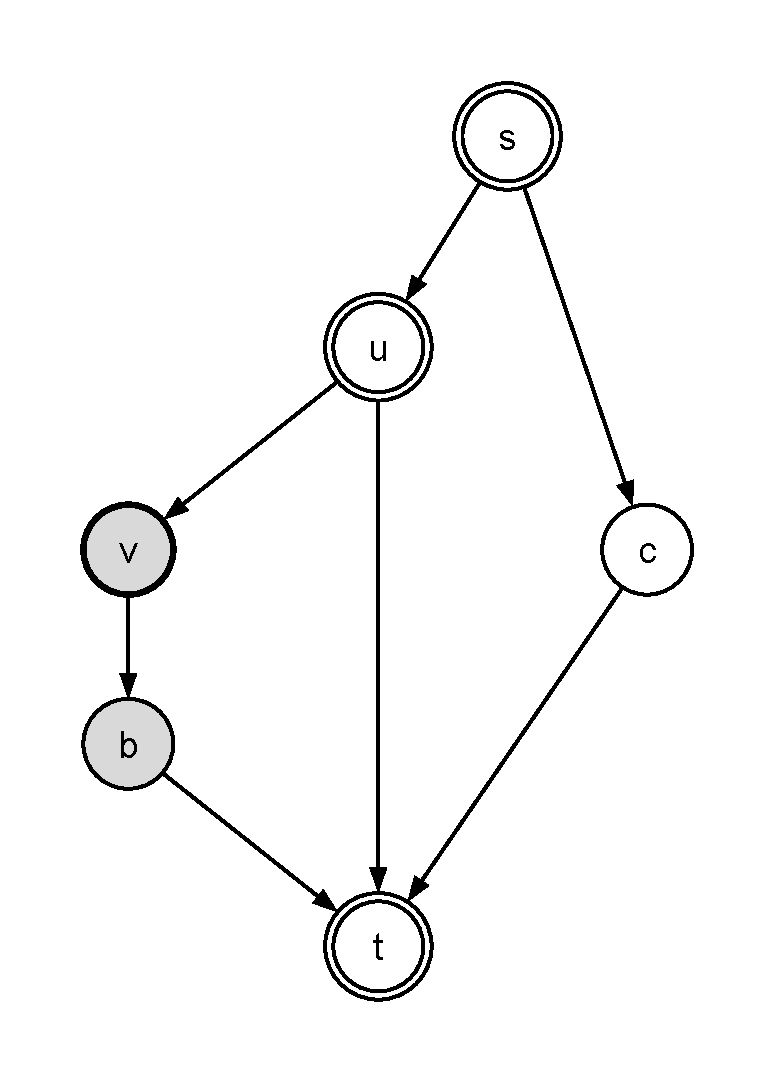
\includegraphics[width=0.5\linewidth]{fig02_bypass/fig02_bypass.pdf}
  \caption{Duration classes relative to node $v$. Shaded nodes are dominated by $v$ (every
  complete route through them passes $v$), the unfilled node is incomparable to it, and
  double-bordered nodes form the bypass set $H_v$: they share routes with $v$ and can also
  route around it.}
  \label{fig:cpm-bypass}
\end{figure}

\begin{theorem}[Exactness of the domination split]
\label{thm:cpm-split}
The maximum of $f_v$ over the box is attained at a corner with every incomparable
duration at its upper bound, every dominated duration at its lower bound, and the bypass
durations at some corner of $H_v$. The minimum is attained dually. Enumerating the
$2^{|H_v|}$ bypass corners with the remaining durations pinned therefore yields the exact
float range of $v$.
\end{theorem}

\begin{proof}
By Proposition~\ref{prop:cpm-corner} an optimum lies at a corner. The three classes
partition the durations. At an optimal corner, moving an incomparable duration to its
upper bound cannot decrease the maximum by Lemma~\ref{lem:cpm-incomparable}, and moving a
dominated duration to its lower bound cannot decrease it by
Lemma~\ref{lem:cpm-dominated}, so some optimal corner has the pinned pattern and lies
within the enumerated set.
\end{proof}

Algorithm~\ref{alg:cpm-split} gives the procedure. Its cost is
\begin{equation}
\label{eq:cpm-split-cost}
2 \sum_{v} 2^{|H_v|}
\end{equation}
scalar propagations, one maximising and one minimising sweep per node, against $2^k$ for
exhaustive enumeration of all $k$ interval durations. The exponent has moved from the size
of the problem to the reconvergent width around each node. One exhaustive sweep serves
every node at once, so the implementation computes both counts before running anything
and uses whichever is cheaper. It is therefore never worse than exhaustive enumeration,
and it refuses when both counts exceed a stated limit. Some instances must remain hard,
because the general problem is NP-hard \cite{chanas2002complexity}, and the split shows
where the hardness sits, in networks whose bypass sets are large.

\begin{algorithm}[htbp]
\caption{Domination split for exact interval floats (LongestPath, point-valued edge values)}
\label{alg:cpm-split}
\begin{algorithmic}[1]
\Require graph object, interval durations $[\underline{d}_u, \overline{d}_u]$, scalar edge
  values, run limit
\Ensure exact float range $[\underline{f}_v, \overline{f}_v]$ for every node $v$
\State $K \gets$ set of nodes with non-degenerate intervals; $k \gets |K|$
\ForAll{nodes $v$}
  \State classify each $u \in K$ as incomparable, dominated, or bypass ($u \in H_v$)
\EndFor
\State total $\gets 2\sum_v 2^{|H_v|}$
\If{$2^k \le$ total} run exhaustive enumeration instead and return \EndIf
\If{total $>$ run limit} refuse \EndIf
\ForAll{nodes $v$}
  \For{objective in (maximise, minimise)}
    \State pin incomparable durations at upper (resp.\ lower) and dominated at lower (resp.\ upper)
    \ForAll{corners of $H_v$}
      \State run Algorithm~\ref{alg:cpm-order}; record $f_v$
    \EndFor
  \EndFor
  \State $\underline{f}_v \gets$ minimum recorded; \quad $\overline{f}_v \gets$ maximum recorded
\EndFor
\State necessarily critical $\gets \{v : \overline{f}_v = 0\}$; \quad possibly critical $\gets \{v : \underline{f}_v = 0\}$
\end{algorithmic}
\end{algorithm}

The bypass set is a measure of reconvergence, and this is where the toolkit meets the
structural theme of Chapter~\ref{ch:diamond-module} without using its module. Both
analyses pay for routes that divide and meet again, the decomposition module per join
through the nodes it must fix, and the split per node through $H_v$. The two sets index
reconvergence at different granularities, neither contains the other in general, and
neither computation uses the other.

\section{Validation}
\label{sec:cpm-validation}

The toolkit was checked against three computations that do not use its kernels. The
checks were run on a set of ten networks, listed with their sizes in
Appendix~\ref{app:full-results}, and they apply to every result reported in
Section~\ref{sec:cpm-cases}.

The first check is a path oracle. It lists every complete path from a source to a sink,
evaluates each path under the mode's operators, and from the list obtains the project
value, the best path through each node, each node's margin and the critical set. On the
seven networks small enough to list every path (32 to 306 nodes, 128 to 2,450 paths), the
toolkit and the oracle agree to within $3 \times 10^{-14}$ in every quantity for all four
modes, and the critical sets are identical. On the three networks with too many paths to
list ($2.7 \times 10^{6}$ and more), two weaker checks are used instead: two thousand
randomly sampled paths never give a better value than the project value the toolkit
reports, and the accumulation total equals the sum of Eq.~\eqref{eq:cpm-acc-total}
evaluated from the multiplicities.

The second check is for the interval methods. The path oracle is run at every corner of
the input box, which gives the exact margin range directly. The conservative enclosure of
Eq.~\eqref{eq:cpm-enclosure} is checked to contain that range, the exhaustive method is
checked to equal it, and the domination split is checked to give the same margins and the
same necessarily and possibly critical sets as the exhaustive method on every network on
which both can run.

The third check is Monte Carlo sampling, used where the exhaustive method is out of
reach. Fifty thousand configurations of durations are drawn uniformly from the box, the
scalar kernel is run on each, and the resulting floats are checked to lie within the
split's bounds and to reach them.

\section{Case Studies}
\label{sec:cpm-cases}

Timings in this section are wall-clock measurements on a single core of the second call
in a warm process, so that just-in-time compilation is excluded. The convention is stated
in Appendix~\ref{app:full-results}.

\subsection{A benchmark project network}
\label{sec:cpm-psplib}

The first case study is instance j301\_1 of the PSPLIB project scheduling library
\cite{kolisch1997psplib}. PSPLIB instances are activity-on-node networks with a dummy start
and a dummy end, each activity carrying a published duration, and they are the standard
benchmark set for project scheduling. The instance has 32 nodes, of which 30 are real
activities, and 48 precedence edges, with one source, one sink, twelve forks and twelve
joins in eleven layers. Its resource requirements are not used: the toolkit computes the
precedence-only schedule, which the PSPLIB instance file records as the MPM-Time of the
instance. The durations are listed in Appendix~\ref{app:network-specs}.

Under LongestPath the project completes in 38 units, which matches the MPM-Time of 38
published with the instance, along the chain
$1 \to 3 \to 8 \to 12 \to 14 \to 17 \to 22 \to 23 \to 24 \to 30 \to 32$
(Figure~\ref{fig:cpm-psplib}). Eleven nodes are critical, nine of them real activities,
and three further activities (4, 10 and 16) carry a slack of one unit
(Table~\ref{tab:cpm-psplib-longest}). Under ShortestPath the fastest complete chain takes
18 units, through activities 2, 4, 6, 10, 25 and 30. The two readings share activity 30 and
nothing else, so the chain that bounds the project from above and the chain that bounds it
from below run through different parts of the network. Each of the three deterministic
passes completes in under 0.2 milliseconds.

\begin{figure}[htbp]
  \centering
  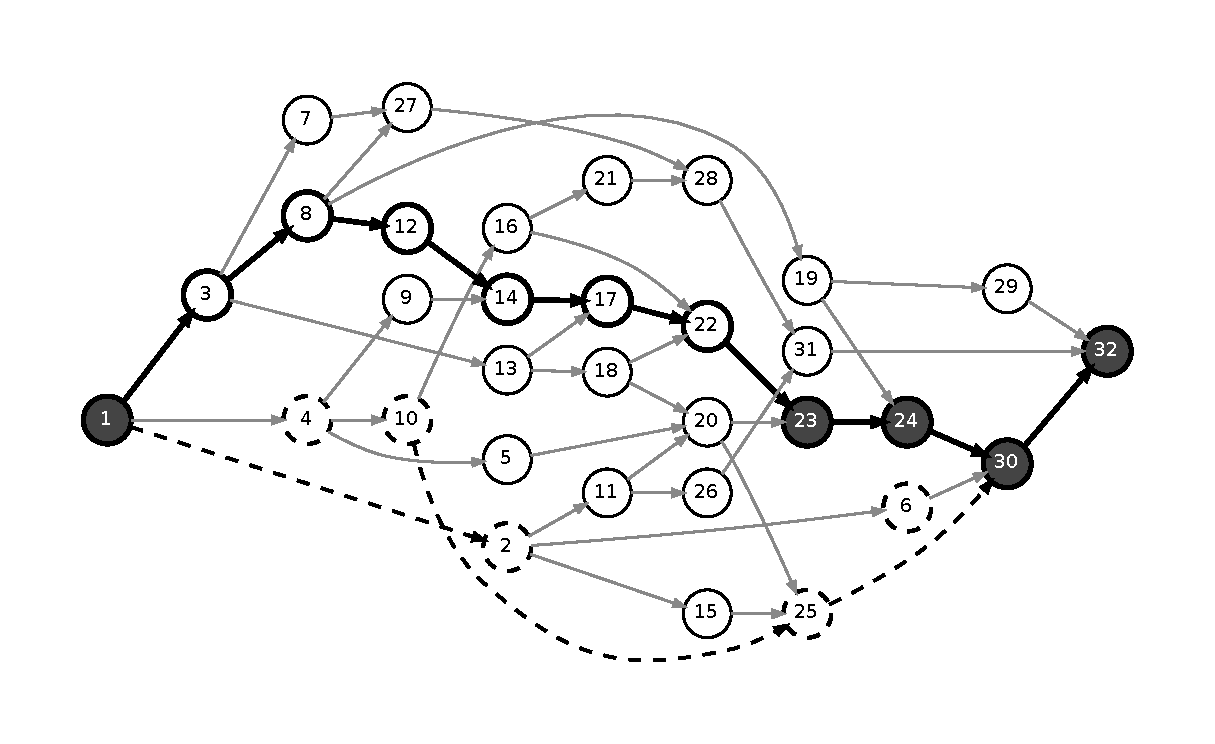
\includegraphics[width=0.9\linewidth]{fig03_psplib/fig03_psplib.pdf}
  \caption{PSPLIB j301\_1. Bold nodes and edges form the LongestPath critical chain
  (completion 38); dashed nodes and edges form the ShortestPath chain (completion 18). The
  filled nodes are those the interval analysis of Figure~\ref{fig:cpm-floats} finds
  necessarily critical under $\pm 20$ per cent duration uncertainty.}
  \label{fig:cpm-psplib}
\end{figure}

\begin{table}[htbp]
\centering
\caption{LongestPath on PSPLIB j301\_1: the critical chain and the three nearest
non-critical activities.}
\label{tab:cpm-psplib-longest}
\small
\renewcommand{\arraystretch}{1.15}
\begin{tabular}{llll}
\toprule
Node & Duration & Completion & Slack \\
\midrule
3  & 4 & 4  & 0 \\
8  & 9 & 13 & 0 \\
12 & 2 & 15 & 0 \\
14 & 3 & 18 & 0 \\
17 & 6 & 24 & 0 \\
22 & 7 & 31 & 0 \\
23 & 2 & 33 & 0 \\
24 & 3 & 36 & 0 \\
30 & 2 & 38 & 0 \\
4  & 6 & 6  & 1 \\
10 & 7 & 13 & 1 \\
16 & 10 & 23 & 1 \\
\bottomrule
\end{tabular}
\end{table}

Read as cost with the same values, the accumulation mode gives a total of 362 at the end
node. The activities with the largest contribution are not those with the largest
durations. Activity 2, with duration 8, reaches the end node along five routes and
contributes 40; activity 3, with duration 4, reaches it along nine routes and contributes
36; activity 16, with duration 10, lies on only two routes and contributes 20
(Table~\ref{tab:cpm-psplib-allowance}). Under a budget of 398.2, ten per cent above the
current total, activity 3 can grow by 4.0 units before the budget is reached, activity 16
by 18.1, and activity 6, which lies on a single route, by 36.2. Contribution and allowance
order the activities differently.

\begin{table}[htbp]
\centering
\caption{Accumulation on PSPLIB j301\_1 under a budget of 398.2 at the end node (current
total 362). Allowance is headroom divided by path multiplicity.}
\label{tab:cpm-psplib-allowance}
\small
\renewcommand{\arraystretch}{1.15}
\begin{tabular}{lllll}
\toprule
Node & Duration & Multiplicity & Contribution & Allowance \\
\midrule
2  & 8  & 5 & 40 & 7.2 \\
3  & 4  & 9 & 36 & 4.0 \\
4  & 6  & 6 & 36 & 6.0 \\
8  & 9  & 4 & 36 & 9.1 \\
11 & 9  & 3 & 27 & 12.1 \\
13 & 6  & 4 & 24 & 9.1 \\
10 & 7  & 3 & 21 & 12.1 \\
16 & 10 & 2 & 20 & 18.1 \\
\bottomrule
\end{tabular}
\end{table}

With every one of the 30 activity durations widened to $\pm 20$ per cent and the two
dummies held at zero, the project value lies in $[30.4, 45.6]$. Exhaustive corner
enumeration of the floats would require $2^{30}$ propagations, about $1.1 \times 10^{9}$.
The domination split required 50,524, a factor of about 21,000 fewer, with the largest
bypass set holding 13 of the 30 durations and the mean bypass set 6.8. It completed in
4.2 seconds, about 82 microseconds per corner, each corner being one run of
Algorithm~\ref{alg:cpm-order}. Five nodes are necessarily critical,
the two dummies and activities 23, 24 and 30, so the final three activities of the
deterministic chain are critical in every configuration of the box while the first six are
not. Nineteen nodes are possibly critical, and thirteen activities cannot become critical
anywhere in the box (Figure~\ref{fig:cpm-floats}).

The conservative enclosure of Section~\ref{sec:cpm-interval}, obtained from the two corner
runs alone, certifies no node as necessarily critical and reports 26 nodes as possibly
critical. The exact split therefore identifies three necessarily critical activities that the
enclosure does not, and removes seven activities from the possibly critical set. The
deterministic pass names eleven nodes, the enclosure names 26, and the exact interval
analysis names 19 and identifies the three that are certain. Monte Carlo sampling of fifty thousand configurations within the box produced no
violation of the bounds. The sampled floats reached the lower and the upper bound at 30 of
the 32 nodes, and at the remaining two the bounds are attained by the corner configurations
the split itself identified.

\begin{figure}[htbp]
  \centering
  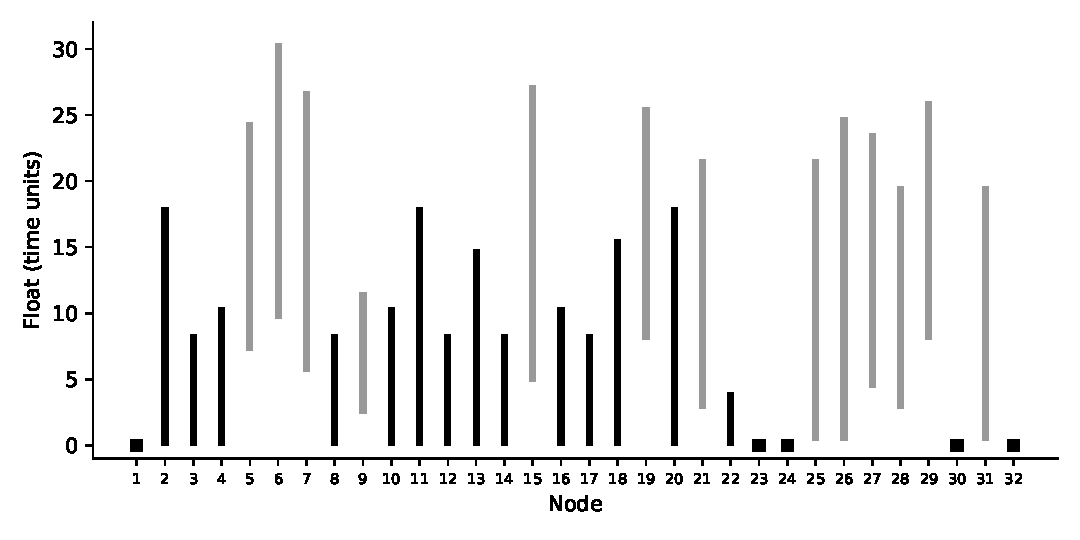
\includegraphics[width=0.75\linewidth]{fig04_floats/fig04_floats.pdf}
  \caption{Exact float bounds on PSPLIB j301\_1 with every duration at plus or minus
  20 per cent. Black bars are the nineteen possibly critical nodes, whose lower bounds
  reach zero; three real activities and the two dummies have upper bound zero as well and
  are necessarily critical. Grey bars are the thirteen activities whose floats stay
  positive everywhere in the box. The five necessarily critical nodes are drawn as points
  at zero, since both bounds of their float are zero.}
  \label{fig:cpm-floats}
\end{figure}

% ---------------------------------------------------------------------------------------
% Former first case study: the bnlearn "water" Bayesian network (Jensen et al. 1989),
% 32 nodes, 66 edges, read with assigned durations. Retained here in case the interval
% result (2^32 vs 2,269,328 runs, max |H_v| = 18) is wanted as a second data point in
% Appendix B. Not a schedule network; do not present as one.
%
% LongestPath: P = 45 along 3 -> 11 -> 19 -> 27; second chain 6 -> 14 -> 22 -> 30 at 1.5
% behind; stage 6 slack 1.0. ShortestPath: P = 15 with twelve margin-zero stages and
% eighteen tight dependencies from three of the eight sources. Accumulation: total 480 at
% outlet 27; stages 3, 6, 5 on seven routes each, allowance +6.9 under budget 528; stage 14
% on two routes, allowance +24. Interval: 2^32 exhaustive vs 2,269,328 split runs (factor
% 1,892), max |H_v| = 18 of 32, mean 10.44; no stage necessarily critical, nine possibly
% critical, 23 provably never critical; MC 50,000 samples, no violation, all bounds
% attained; split 307 s at 135 us per run.
% ---------------------------------------------------------------------------------------

\subsection{The boundary of the split}
\label{sec:cpm-boundary}

The advantage of the split disappears under dense mesh reconvergence. On a five-by-five
grid DAG with all 25 durations interval-valued, the bypass sets hold up to 23 of the 25
durations, so the split would need $3.9 \times 10^{7}$ propagations against
$3.4 \times 10^{7}$ for one shared exhaustive sweep. The never-worse rule therefore
selects the exhaustive sweep, and the instance is at the boundary of the method. The
hardness results guarantee that some regime behaves this way, and it is the same regime
in which the conditioning sets of the probability toolkit grow.

\section{Discussion}
\label{sec:cpm-discussion}

The domination split is proved and implemented for the LongestPath mode only. The
ShortestPath dual mirrors Section~\ref{sec:cpm-split} but has not been derived in full,
and the toolkit refuses the split for any other mode. For those modes the exact interval
margins are available only by exhaustive corner enumeration.

The split requires point-valued edge values. An interval-valued edge reduces to an interval
duration by subdividing the edge with a node that carries the value, so the reduction is
known, but the toolkit does not yet perform it and refuses interval edge values on the
split path.

Probability-box durations are not supported. The forward quantities would propagate by the
p-box arithmetic of Chapter~\ref{ch:lit-review}, but the margins would meet the same
dependence problem as the intervals, and no corner argument applies to them. Therefore no
method for them is claimed.

The cost of the split grows with the bypass sets, and on dense meshes the sets approach the
whole network. The never-worse rule keeps the cost at or below that of exhaustive enumeration, and no lower.

The boundary of the toolkit is set by the algebra. A new
quantity is added by giving its operator pair, and the pair obtains a backward pass in the
same way as the four provided modes, by carrying a residual or by being linear. Whether a
proposed pair has this property is a mathematical question that the implementation does
not check, and showing it is the responsibility of whoever adds the mode. Two extensions
follow the existing arguments: neighbouring nodes have overlapping bypass sets and
therefore overlapping corner evaluations, which could be shared in the way the hash-consed
store of Chapter~\ref{ch:diamond-module} shares diamonds, and the edge subdivision above
would admit interval edge values. These are listed in Chapter~\ref{ch:conclusions}.

\section{Summary}
\label{sec:cpm-summary}

In this chapter the Critical Path Toolkit has been presented. The classical critical path
method has been generalised to a family of analysis modes, each an operator pair with the
backward semantics its algebra supports, and four modes have been provided: LongestPath,
ShortestPath and MaxScaling on one order-based kernel, and Accumulation on a linear kernel
whose backward object is the adjoint. Under interval durations the forward quantities have
been computed exactly from two scalar runs, and the floats exactly by the domination split,
whose correctness rests on three short proofs and whose cost grows with the reconvergent
width around each node instead of with the number of uncertain inputs. The toolkit has been
validated against a path oracle, exhaustive corner enumeration and Monte Carlo sampling,
and applied to a benchmark project network. The MaxScaling mode is demonstrated on the
integrated case study of Chapter~\ref{ch:integrated-case-study}. On a dense mesh the split reaches its boundary and the toolkit falls back to exhaustive
enumeration, as the hardness of the general problem requires.

\ifdefined\maindoc
% do nothing
\else
\printbibliography
\end{document}
\fi